
%\documentclass[11pts,a4paper,amsmath,amssymb,floatfix]{article}%{report}%{book}
\documentclass[12pts,a4paper,amsmath,amssymb,floatfix]{article}%{report}%{book}
\usepackage{graphicx,wrapfig,pdfpages}% Include figure files
%\usepackage{dcolumn,enumerate}% Align table columns on decimal point
\usepackage{enumerate,enumitem}% Align table columns on decimal point
\usepackage{bm,dpfloat}% bold math
\usepackage[pdftex,bookmarks,colorlinks=true,urlcolor=rltblue,citecolor=blue]{hyperref}
\usepackage{amsfonts,amsmath,amssymb,stmaryrd,indentfirst}
\usepackage{times,psfrag}
\usepackage{natbib}
\usepackage{color}
\usepackage{units}
\usepackage{rotating}
\usepackage{multirow}


\usepackage{pifont}
\usepackage{subfigure}
\usepackage{subeqnarray}
\usepackage{ifthen}

\usepackage{supertabular}
\usepackage{moreverb}
\usepackage{listings}
\usepackage{palatino}
%\usepackage{doi}
\usepackage{longtable}
\usepackage{float}
\usepackage{perpage}
\MakeSorted{figure}
%\usepackage{pdflscape}


%\usepackage{booktabs}
%\newcommand{\ra}[1]{\renewcommand{\arraystretch}{#1}}


\definecolor{rltblue}{rgb}{0,0,0.75}


%\usepackage{natbib}
\usepackage{fancyhdr} %%%%
\pagestyle{fancy}%%%%
% with this we ensure that the chapter and section
% headings are in lowercase
%%%%\renewcommand{\chaptermark}[1]{\markboth{#1}{}}
\renewcommand{\sectionmark}[1]{\markright{\thesection\ #1}}
\fancyhf{} %delete the current section for header and footer
\fancyhead[LE,RO]{\bfseries\thepage}
\fancyhead[LO]{\bfseries\rightmark}
\fancyhead[RE]{\bfseries\leftmark}
\renewcommand{\headrulewidth}{0.5pt}
% make space for the rule
\fancypagestyle{plain}{%
\fancyhead{} %get rid of the headers on plain pages
\renewcommand{\headrulewidth}{0pt} % and the line
}

\def\newblock{\hskip .11em plus .33em minus .07em}
\usepackage{color}

%\usepackage{makeidx}
%\makeindex

\setlength\textwidth      {16.cm}
\setlength\textheight     {22.6cm}
\setlength\oddsidemargin  {-0.3cm}
\setlength\evensidemargin {0.3cm}

\setlength\headheight{14.49998pt} 
\setlength\topmargin{0.0cm}
\setlength\headsep{1.cm}
\setlength\footskip{1.cm}
\setlength\parskip{0pt}
\setlength\parindent{0pt}


%%%
%%% Headers and Footers
\lhead[] {\text{\small{EX3029 -- Chemical Thermodynamics}}} 
\rhead[] {{\text{\small{Tutorial 01 (2014/15)}}}}
%\chead[] {\text{\small{Session 2012/13}}} 
\lfoot[]{Dr Jeff Gomes}
%\cfoot[\thepage]{\thepage}
\rfoot[\text{\small{\thepage}}]{\thepage}
\renewcommand{\headrulewidth}{0.8pt}


%%%
%%% space between lines
%%%
\renewcommand{\baselinestretch}{1.5}

\newenvironment{VarDescription}[1]%
  {\begin{list}{}{\renewcommand{\makelabel}[1]{\textbf{##1:}\hfil}%
    \settowidth{\labelwidth}{\textbf{#1:}}%
    \setlength{\leftmargin}{\labelwidth}\addtolength{\leftmargin}{\labelsep}}}%
  {\end{list}}

%%%%%%%%%%%%%%%%%%%%%%%%%%%%%%%%%%%%%%%%%%%
%%%%%%                              %%%%%%%
%%%%%%      NOTATION SECTION        %%%%%%%
%%%%%%                              %%%%%%%
%%%%%%%%%%%%%%%%%%%%%%%%%%%%%%%%%%%%%%%%%%%

% Text abbreviations.
\newcommand{\ie}{{\em{i.e., }}}
\newcommand{\eg}{{\em{e.g., }}}
\newcommand{\cf}{{\em{cf., }}}
\newcommand{\wrt}{with respect to}
\newcommand{\lhs}{left hand side}
\newcommand{\rhs}{right hand side}
% Commands definining mathematical notation.

% This is for quantities which are physically vectors.
\renewcommand{\vec}[1]{{\mbox{\boldmath$#1$}}}
% Physical rank 2 tensors
\newcommand{\tensor}[1]{\overline{\overline{#1}}}
% This is for vectors formed of the value of a quantity at each node.
\newcommand{\dvec}[1]{\underline{#1}}
% This is for matrices in the discrete system.
\newcommand{\mat}[1]{\mathrm{#1}}


\DeclareMathOperator{\sgn}{sgn}
\newtheorem{thm}{Theorem}[section]
\newtheorem{lemma}[thm]{Lemma}

%\newcommand\qed{\hfill\mbox{$\Box$}}
\newcommand{\re}{{\mathrm{I}\hspace{-0.2em}\mathrm{R}}}
\newcommand{\inner}[2]{\langle#1,#2\rangle}
\renewcommand\leq{\leqslant}
\renewcommand\geq{\geqslant}
\renewcommand\le{\leqslant}
\renewcommand\ge{\geqslant}
\renewcommand\epsilon{\varepsilon}
\newcommand\eps{\varepsilon}
\renewcommand\phi{\varphi}
\newcommand{\bmF}{\vec{F}}
\newcommand{\bmphi}{\vec{\phi}}
\newcommand{\bmn}{\vec{n}}
\newcommand{\bmns}{{\textrm{\scriptsize{\boldmath $n$}}}}
\newcommand{\bmi}{\vec{i}}
\newcommand{\bmj}{\vec{j}}
\newcommand{\bmk}{\vec{k}}
\newcommand{\bmx}{\vec{x}}
\newcommand{\bmu}{\vec{u}}
\newcommand{\bmv}{\vec{v}}
\newcommand{\bmr}{\vec{r}}
\newcommand{\bma}{\vec{a}}
\newcommand{\bmg}{\vec{g}}
\newcommand{\bmU}{\vec{U}}
\newcommand{\bmI}{\vec{I}}
\newcommand{\bmq}{\vec{q}}
\newcommand{\bmT}{\vec{T}}
\newcommand{\bmM}{\vec{M}}
\newcommand{\bmtau}{\vec{\tau}}
\newcommand{\bmOmega}{\vec{\Omega}}
\newcommand{\pp}{\partial}
\newcommand{\kaptens}{\tensor{\kappa}}
\newcommand{\tautens}{\tensor{\tau}}
\newcommand{\sigtens}{\tensor{\sigma}}
\newcommand{\etens}{\tensor{\dot\epsilon}}
\newcommand{\ktens}{\tensor{k}}
\newcommand{\half}{{\textstyle \frac{1}{2}}}
\newcommand{\tote}{E}
\newcommand{\inte}{e}
\newcommand{\strt}{\dot\epsilon}
\newcommand{\modu}{|\bmu|}
% Derivatives
\renewcommand{\d}{\mathrm{d}}
\newcommand{\D}{\mathrm{D}}
\newcommand{\ddx}[2][x]{\frac{\d#2}{\d#1}}
\newcommand{\ddxx}[2][x]{\frac{\d^2#2}{\d#1^2}}
\newcommand{\ddt}[2][t]{\frac{\d#2}{\d#1}}
\newcommand{\ddtt}[2][t]{\frac{\d^2#2}{\d#1^2}}
\newcommand{\ppx}[2][x]{\frac{\partial#2}{\partial#1}}
\newcommand{\ppxx}[2][x]{\frac{\partial^2#2}{\partial#1^2}}
\newcommand{\ppt}[2][t]{\frac{\partial#2}{\partial#1}}
\newcommand{\pptt}[2][t]{\frac{\partial^2#2}{\partial#1^2}}
\newcommand{\DDx}[2][x]{\frac{\D#2}{\D#1}}
\newcommand{\DDxx}[2][x]{\frac{\D^2#2}{\D#1^2}}
\newcommand{\DDt}[2][t]{\frac{\D#2}{\D#1}}
\newcommand{\DDtt}[2][t]{\frac{\D^2#2}{\D#1^2}}
% Norms
\newcommand{\Ltwo}{\ensuremath{L_2} }
% Basis functions
\newcommand{\Qone}{\ensuremath{Q_1} }
\newcommand{\Qtwo}{\ensuremath{Q_2} }
\newcommand{\Qthree}{\ensuremath{Q_3} }
\newcommand{\QN}{\ensuremath{Q_N} }
\newcommand{\Pzero}{\ensuremath{P_0} }
\newcommand{\Pone}{\ensuremath{P_1} }
\newcommand{\Ptwo}{\ensuremath{P_2} }
\newcommand{\Pthree}{\ensuremath{P_3} }
\newcommand{\PN}{\ensuremath{P_N} }
\newcommand{\Poo}{\ensuremath{P_1P_1} }
\newcommand{\PoDGPt}{\ensuremath{P_{-1}P_2} }

\newcommand{\metric}{\tensor{M}}
\newcommand{\configureflag}[1]{\texttt{#1}}

% Units
\newcommand{\m}[1][]{\unit[#1]{m}}
\newcommand{\km}[1][]{\unit[#1]{km}}
\newcommand{\s}[1][]{\unit[#1]{s}}
\newcommand{\invs}[1][]{\unit[#1]{s}\ensuremath{^{-1}}}
\newcommand{\ms}[1][]{\unit[#1]{m\ensuremath{\,}s\ensuremath{^{-1}}}}
\newcommand{\mss}[1][]{\unit[#1]{m\ensuremath{\,}s\ensuremath{^{-2}}}}
\newcommand{\K}[1][]{\unit[#1]{K}}
\newcommand{\PSU}[1][]{\unit[#1]{PSU}}
\newcommand{\Pa}[1][]{\unit[#1]{Pa}}
\newcommand{\kg}[1][]{\unit[#1]{kg}}
\newcommand{\rads}[1][]{\unit[#1]{rad\ensuremath{\,}s\ensuremath{^{-1}}}}
\newcommand{\kgmm}[1][]{\unit[#1]{kg\ensuremath{\,}m\ensuremath{^{-2}}}}
\newcommand{\kgmmm}[1][]{\unit[#1]{kg\ensuremath{\,}m\ensuremath{^{-3}}}}
\newcommand{\Nmm}[1][]{\unit[#1]{N\ensuremath{\,}m\ensuremath{^{-2}}}}

% Dimensionless numbers
\newcommand{\dimensionless}[1]{\mathrm{#1}}
\renewcommand{\Re}{\dimensionless{Re}}
\newcommand{\Ro}{\dimensionless{Ro}}
\newcommand{\Fr}{\dimensionless{Fr}}
\newcommand{\Bu}{\dimensionless{Bu}}
\newcommand{\Ri}{\dimensionless{Ri}}
\renewcommand{\Pr}{\dimensionless{Pr}}
\newcommand{\Pe}{\dimensionless{Pe}}
\newcommand{\Ek}{\dimensionless{Ek}}
\newcommand{\Gr}{\dimensionless{Gr}}
\newcommand{\Ra}{\dimensionless{Ra}}
\newcommand{\Sh}{\dimensionless{Sh}}
\newcommand{\Sc}{\dimensionless{Sc}}


% Journals
\newcommand{\IJHMT}{{\it International Journal of Heat and Mass Transfer}}
\newcommand{\NED}{{\it Nuclear Engineering and Design}}
\newcommand{\ICHMT}{{\it International Communications in Heat and Mass Transfer}}
\newcommand{\NET}{{\it Nuclear Engineering and Technology}}
\newcommand{\HT}{{\it Heat Transfer}}   
\newcommand{\IJHT}{{\it International Journal for Heat Transfer}}

\newcommand{\frc}{\displaystyle\frac}

\newlist{ExList}{enumerate}{1}
\setlist[ExList,1]{label={\bf Example 1.} {\bf \arabic*}}

\newlist{ProbList}{enumerate}{1}
\setlist[ProbList,1]{label={\bf Problem 1.} {\bf \arabic*}}

%%%%%%%%%%%%%%%%%%%%%%%%%%%%%%%%%%%%%%%%%%%
%%%%%%                              %%%%%%%
%%%%%% END OF THE NOTATION SECTION  %%%%%%%
%%%%%%                              %%%%%%%
%%%%%%%%%%%%%%%%%%%%%%%%%%%%%%%%%%%%%%%%%%%


% Cause numbering of subsubsections. 
%\setcounter{secnumdepth}{8}
%\setcounter{tocdepth}{8}

\setcounter{secnumdepth}{4}%
\setcounter{tocdepth}{4}%


\begin{document}



\begin{enumerate}[label=\bfseries Problem \arabic*:]

%%%
%%%
%%%
\item\label{Tut01:UnitConversion} A closed system contains 1 mol of nitrogen $\left(\text{MW = 28 g. mol}^{-1}\right)$. Using the ideal gas law, calculate the missing {\it PVT} parameter for the following data given. Give your results in {\bf SI units}. The universal gas constant is $\text{R = 8.314 J.gmol}^{-1}\text{.K}^{-1}$.
\begin{enumerate}   
\item P = 1 atm, T = 0$^{\circ}$C
\item V$^{t}$ = 12.85 ft$^{3}$; T = 59$^{\circ}$F
\item P = 2.5$\times$10$^{9}$ g.m$^{-1}$.s$^{-2}$; T = 650.50$^{\circ}$R
\item V$^{t}$ = 1.3$\times$10$^{-12}$Gl; P= 500 psi
\end{enumerate}


%%%
%%%
%%%
\item\label{Tut01:LinearInterpolation} In a coal-fired power station water-steam system is used to produce electricity. Determine the enthalpy $\left(\text{kJ.kg}^{-1}\right)$ and entropy $\left(\text{kJ.kg}^{-1}.K^{-1}\right)$ of the system under the following conditions (a-h):
\begin{center}
\begin{tabular}{||c | c |  c  c | c ||}
\hline\hline
{\bf Pressure}  & {\bf Temperature}  & {\bf Enthalpy}      & {\bf Entropy}               &   {\bf State} \\
{\bf (bar)}     &                    & {\bf kJ.kg$^{-1}$}   & {\bf kJ.kg$^{-1}$.K$^{-1}$}  &               \\
\hline
 150.0          &    733.15 K        &     (a)             &     (b)                     &   (c)         \\
  37.5          &     --             &     (d)             &     (e)                     &   liquid water \\
 142.6          &    375.00$^{\circ}$C&     (f)             &     (g)                     &   (h)         \\  
\hline\hline
\end{tabular}
\end{center} 


%%%
%%%
%%%
\item\label{Tut01:PotentialEnergy1} The {\it Angle Falls} in Venezuela are the world’s highest waterfalls ($\sim$1000 m). Take the amount of 1 kg of water as the system flowing over the waterfall. Assume that is does not exchange energy with its surroundings.
\begin{enumerate}
\item Calculate the potential energy of the water at the top of the falls with respect to the base of the falls. Assume gravity acceleration as 9.81 m.s$^{-2}$.
\item What is the energy balance that applies during the water falling down? What is the kinetic energy of the water just before it strikes down?
\item When striking down the energy is converted to internal energy. Calculate the temperature change with the heat capacity 4184 J.kg$^{-1}$.K$^{-1}$.
\end{enumerate}


%%%
%%%
%%%
\item\label{Tut01:PotentialEnergy2} A hydroturbine operates with a head of 160 ft of water. Inlet and outlet conduits are 78.74 inches in diameter. Calculate the maximum mechanical power (in kW) that can be developed by the turbine for an inlet velocity of 18 km.h$^{-1}$.


%%%
%%%
%%%
\item\label{Tut01:FirstLawIdealGas1} Given {\it Ar} at P$_{1}$ = 140 kPa, T$_{1}$ = 10$^{o}$C, V$_{1}$ = 200 liters which undergoes a polytropic compression to P$_{2}$ = 700 kPa, T$_{2}$ = 180 $^{o}$C, find Q$_{1-2}$. Given MW = 39.948 kg.kgmole$^{-1}$, R = 0.2081 kJ.kg$^{-1}$.K$^{-1}$ and C$_{V}$ = 0.312 kJ.kg$^{-1}$.K$^{-1}$.


%%%
%%%
%%%
\item\label{Tut01:FirstLawIdealGas2} Given air (assuming ideal gas behaviour) expanding reversibly and adiabatically from $T_{1}=450 K$ and $V_{1}=3.0\times 10^{-3}m^{3}$ to the final volume, $V_{2}=5.0\times 10^{-3}m^{3}$. $T$ and $V$ relationship for constant heat capacities is represented by $\displaystyle\frc{T_{2}}{T_{1}} = \left(\frc{V_{1}}{V_{2}}\right)^{\gamma-1}$.
\begin{enumerate}
\item Derive a relationship between $T$ and $P$; Assuming that $C_{p}= 5.0 cal.\left(mol.K\right)^{-1}$ and $C_{v}=3.0 cal.\left(mol.K\right)^{-1}$;
\item Calculate $T_{2}$;
\item Calculate the work done during the process and;
\item Determine the enthalpy change.
\end{enumerate}

%%%
%%% Problem 2.69 (Saphiro)
%%%
\item\label{Tut01:FirstLawIdealGas3} Gaseous CO$_{2}$ $\left(\text{m}_{CO_{2}}=4g\right)$ is contained in a vertical piston-cylinder assembly by a piston of mass 50 kg and having a face area of 1.0$\times$10$^{-2}$m$^{2}$. The CO$_{2}$ initially occupies a volume of 5$\times$10$^{-3}$m$^{3}$ and has a specific internal energy of 657 kJ.kg$^{-1}$.  The atmosphere exerts a pressure of 100 kPa on the top of the piston. Heat transfer in the amount  of 1.95 kJ occurs slowly from the CO$_{2}$ to the surroundings, and the volume of the CO$_{2}$ decreases to 2.5$\times$10$^{-3}$m$^{3}$. Friction between the piston and the cylinder wall can be neglected. The local acceleration of gravity is 9.81 m.s$^{-2}$. For the CO$_{2}$, determine (a) the pressure in kPa and (b) the final specific internal energy in kJ.kg$^{-1}$.

%%%
%%% Problem 2.33 (Saphiro)
%%%
\item\label{Tut01:FirstLawIdealGas3} CO gas contained within a piston-cylinder assembly undergoes three processes in series:
    \begin{itemize}
       \item Process 1-2: expansion from p$_{1}$ = 5 bar, V$_{1}$ = 0.2 m$^{3}$ to V$_{2}$ = 1.0 m$^{3}$, during which the pressure-volume relationship is pV = constant.
       \item Process 2-3: constant volume heating from state 2 to state 3, where p$_{3}$ = 5 bar.
       \item Process 3-1: constant pressure compression to the initial state.
    \end{itemize}
       Sketch the processes in series on p-V coordinates and evaluate the work for each process, in kJ.


\begin{comment}
%%%
%%% Problem 5.78 (Saphiro)
%%%
\item\label{Tut01:FirstLawDerivation}The pressure-volume diagram of a Carnot power cycle executed by an ideal gas with constant specific heat ratio $\kappa$ is shown in Fig. \ref{Prob_Saphiro_5.78}. Demonstrate that: (a) $V_{4}V_{2}=V_{1}V_{3}$, (b) $\frc{T_{2}}{T_{3}} = \left(\frc{P_{2}}{P_{3}}\right)^{\frc{\kappa - 1}{\kappa}}$ and (c) $\frc{T_{2}}{T_{3}}=\left(\frc{V_{3}}{V_{2}}\right)^{\kappa - 1}$
\begin{figure}[h]
\begin{center}
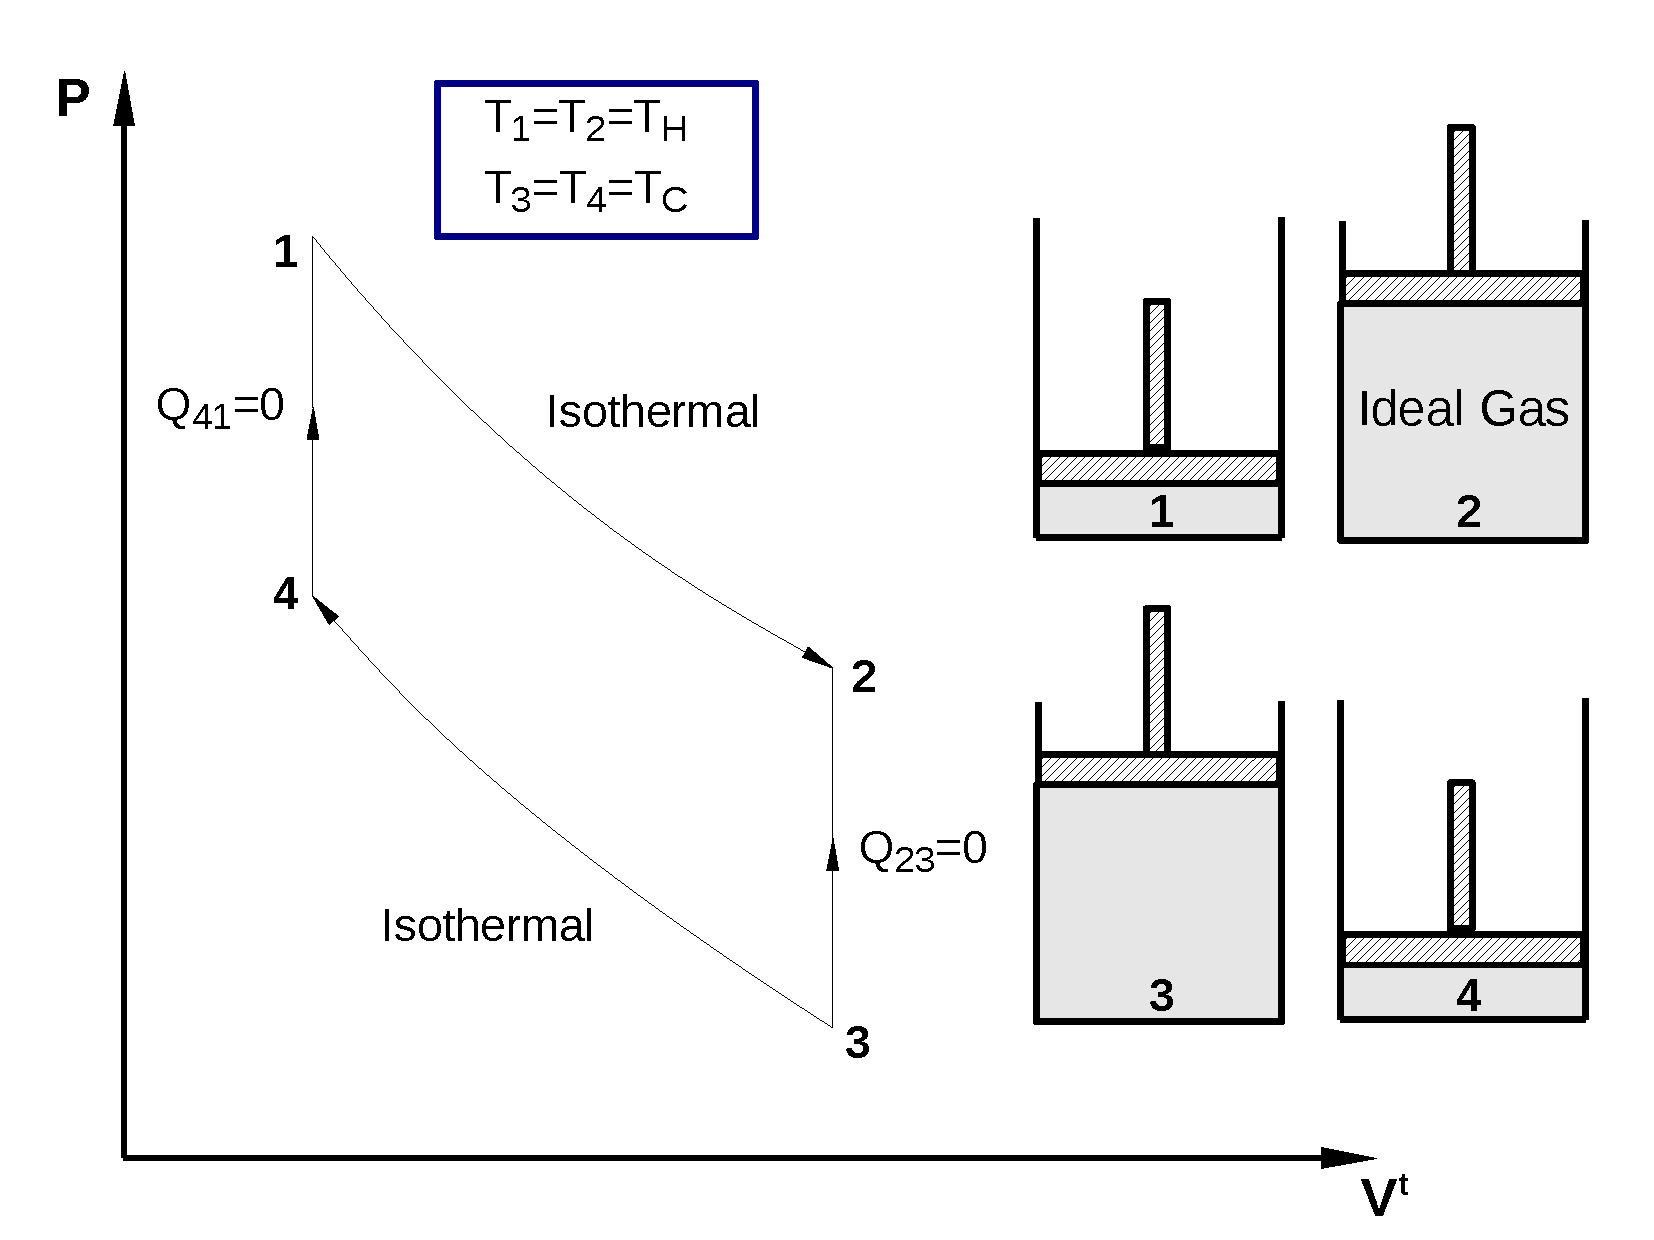
\includegraphics[width=6.cm,clip]{./Pics/Problem_5_78}
\caption{Problem \ref{Tut01:FirstLawDerivation}.}
\label{Prob_Saphiro_5.78}
\end{center}
\end{figure}
\end{comment}

%\begin{comment}
%\end{comment}

\end{enumerate}



\clearpage

%{
%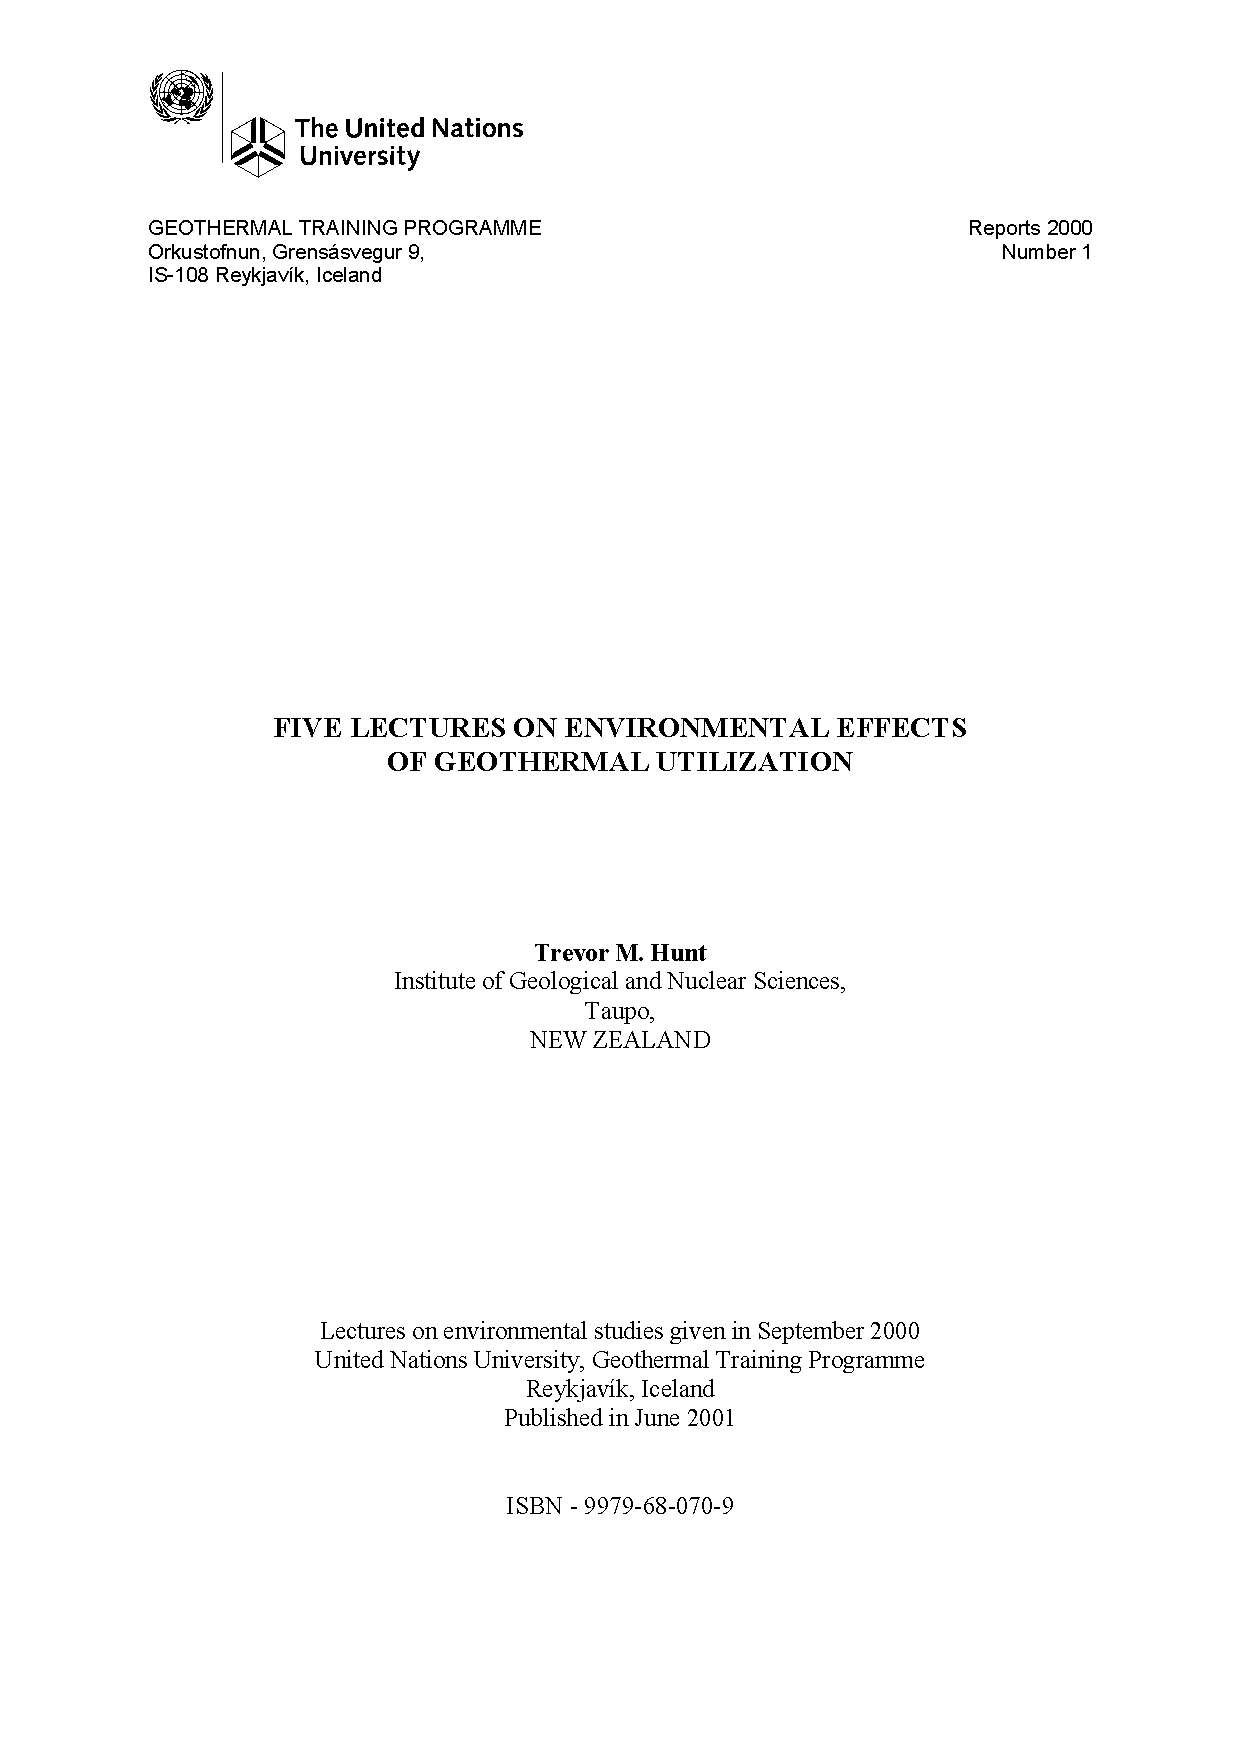
\includepdf[pages=-,fitpaper, angle=0]{./HuntSelect.pdf}
%}

\end{document}
